% =============================================================================
% AIT Thesis/Project Report Format
% Based on Asian Institute of Technology thesis formatting guidelines
% =============================================================================

\documentclass[12pt,a4paper]{report}

% ── AIT margins: 1.5in left (binding), 1in elsewhere ─────────────────────────
\usepackage[a4paper, margin=1in, left=1.5in]{geometry}

% ── AIT font: Times-family serif, 12pt ───────────────────────────────────────
\usepackage[T1]{fontenc}
\usepackage{tgtermes}

% ── AIT line spacing: 1.5 ────────────────────────────────────────────────────
\usepackage{setspace}
\onehalfspacing

% ── standard packages ─────────────────────────────────────────────────────────
\usepackage{amsmath,amssymb,amsthm}
\usepackage{booktabs}
\usepackage{listings}
\usepackage{xcolor}
\usepackage[hidelinks]{hyperref}
\usepackage{enumitem}
\usepackage{caption}
\usepackage{float}
\usepackage{tikz}
\usetikzlibrary{shapes.geometric, arrows.meta, positioning, fit, backgrounds}
\usepackage{microtype}
\usepackage[titles]{tocloft}
\usepackage{fancybox}       % for shadowbox around error output
\usepackage{adjustbox}      % for fitting wide tables

% ── AIT heading styles ───────────────────────────────────────────────────────
\usepackage{titlesec}
\usepackage{xurl}


\renewcommand{\chaptername}{CHAPTER}
\titleformat{\chapter}[display]
  {\centering\large\bfseries}
  {\MakeUppercase{\chaptertitlename}\ \thechapter}{0.5em}
  {\large\bfseries\MakeUppercase}
\titlespacing*{\chapter}{0pt}{-20pt}{20pt}

\titleformat{\section}
  {\normalfont\normalsize\bfseries}{\thesection}{1em}{}
\titlespacing*{\section}{0pt}{12pt plus 2pt}{6pt}

\titleformat{\subsection}
  {\normalfont\normalsize\bfseries\itshape}{\thesubsection}{1em}{}
\titlespacing*{\subsection}{0pt}{12pt plus 2pt}{6pt}

\titleformat{\paragraph}[runin]
  {\normalfont\normalsize\bfseries}{}{0em}{}[.]
\titlespacing*{\paragraph}{0pt}{6pt}{6pt}

% ── AIT paragraph style ──────────────────────────────────────────────────────
\setlength{\parindent}{0pt}
\setlength{\parskip}{12pt}

% ── AIT table of contents formatting ─────────────────────────────────────────
\renewcommand{\cftchapfont}{\bfseries}
\renewcommand{\cftchappagefont}{\bfseries}
\renewcommand{\cftdot}{}
\renewcommand\contentsname{\centering\large\bfseries CONTENTS}
\renewcommand\listfigurename{\centering\large\bfseries LIST OF FIGURES}
\renewcommand\listtablename{\centering\large\bfseries LIST OF TABLES}

% ── AIT caption style ────────────────────────────────────────────────────────
\captionsetup[figure]{labelfont=bf, labelsep=colon, justification=centering, singlelinecheck=true}
\captionsetup[table]{labelfont=bf, name=Table\space}
\captionsetup[figure]{labelfont=bf, name=Figure\space}

% ── listings: plain academic style ───────────────────────────────────────────
\lstdefinelanguage{PL}{
  morekeywords={def,int,float,bool,string,if,then,else,while,do,return,print,true,false},
  sensitive=true,
  morecomment=[l]{\#},
  morestring=[b]",
}

\lstdefinestyle{plstyle}{
  language=PL,
  basicstyle=\ttfamily\small,
  keywordstyle=\bfseries,
  commentstyle=\itshape\color{gray},
  stringstyle=\color{black},
  numberstyle=\tiny\color{gray},
  numbers=left,
  numbersep=10pt,
  breaklines=true,
  frame=lines,
  framesep=4pt,
  xleftmargin=1.5em,
  showstringspaces=false,
  tabsize=4,
  captionpos=b,
  aboveskip=0.8em,
  belowskip=0.8em,
}

\lstdefinestyle{tacstyle}{
  basicstyle=\ttfamily\small,
  numbers=left,
  numberstyle=\tiny\color{gray},
  numbersep=10pt,
  frame=lines,
  framesep=4pt,
  xleftmargin=1.5em,
  breaklines=true,
  captionpos=b,
  aboveskip=0.8em,
  belowskip=0.8em,
}

% ── error output style (framed box) ─────────────────────────────────────────
\lstdefinestyle{errorstyle}{
  basicstyle=\ttfamily\small,
  numbers=none,
  frame=single,
  framesep=6pt,
  xleftmargin=0.5em,
  xrightmargin=0.5em,
  breaklines=true,
  aboveskip=0.8em,
  belowskip=0.8em,
  backgroundcolor=\color{gray!5},
}

\lstset{style=plstyle}

% ── type-rule helpers (smaller to avoid overflow) ────────────────────────────
\newcommand{\typerule}[2]{\dfrac{\displaystyle #1}{\displaystyle #2}}
\newcommand{\typerulesmall}[2]{\frac{#1}{#2}}
\newcommand{\Env}{\Gamma}
\newcommand{\proves}{\vdash}
\newcommand{\tint}{\texttt{int}}
\newcommand{\tfloat}{\texttt{float}}
\newcommand{\tbool}{\texttt{bool}}
\newcommand{\tstring}{\texttt{string}}

% ── TikZ styles ──────────────────────────────────────────────────────────────
\tikzset{
  pipenode/.style={
    rectangle, rounded corners=4pt,
    draw=black, thick,
    minimum width=2.0cm, minimum height=0.8cm,
    text centered, font=\small\sffamily,
    fill=gray!10,
  },
  arrow/.style={-{Stealth[length=6pt]}, thick},
  annot/.style={font=\scriptsize\itshape, text=gray, align=center},
}

\pagestyle{plain}

% =============================================================================
\begin{document}
% =============================================================================

% ── Title Page (AIT Format) ──────────────────────────────────────────────────
\pagenumbering{roman}
\begin{titlepage}
  \centering
  \vspace*{2cm}

  {\large\bfseries A Statically Typed Programming Language\\[0.4em]
  with Type Inference, and Three-Address Code Generation\\[0.4em]
  \par}

  \vspace{1cm}

  {\normalsize by\par}
  \vspace{0.5cm}

  {\large\itshape Yosakorn Sirisoot, Anish Manandhar, Prajwal Bhandary\par}

  \vspace{2cm}

  {\large
  A Project Report Submitted in Partial Fulfillment\\
  of the Requirements for the Course\\[0.5em]
  \textbf{Programming Languages and Compilers}\\[2cm]
  }

  {\large\bfseries Asian Institute of Technology\par}
  \vspace{0.3cm}
  {\normalsize School of Engineering and Technology\par}
  \vspace{0.3cm}

  \vfill
\end{titlepage}

% ── Abstract ─────────────────────────────────────────────────────────────────
\clearpage
\addcontentsline{toc}{chapter}{\bfseries ABSTRACT}
\begin{center}
  {\large\bfseries ABSTRACT}
\end{center}
\vspace{1em}

This report describes the design and implementation of a small,
statically typed programming language that our team has developed.
The language supports four primitive types (\tint, \tfloat, \tbool,
and~\tstring), static typing with first-assignment type inference, arithmetic
and boolean expressions without operator overloading, standard control
structures, and user-defined functions with value-parameter passing.
The implementation covers the full compilation pipeline: lexical analysis,
LALR(1) parsing, type checking with inference, three-address code (TAC)
generation, and interpretation. A browser-based online compiler is also
provided to allow users to write, compile, and execute programs without
local installation.

% ── Table of Contents ────────────────────────────────────────────────────────
\clearpage
\addtocontents{toc}{~\hfill\textbf{Page}\par}
\tableofcontents

% ── List of Figures ──────────────────────────────────────────────────────────
\clearpage
\listoffigures

% ── List of Tables ───────────────────────────────────────────────────────────
\clearpage
\listoftables

% =============================================================================
\clearpage
\pagenumbering{arabic}
% =============================================================================

% =============================================================================
\chapter{Introduction}
% =============================================================================

Programming language implementation is one of the central topics in computer
science education. This project required building a complete runnable
programming language that satisfies a concrete specification: static typing,
no overloading, four base types, the standard imperative control structures,
and user-defined functions with value-parameter passing.

The result is a complete language implementation built entirely in Python~3.12
using the \textit{sly} parser-generator library.\footnote{Source code: \url{https://github.com/prazwal1/plc-project.git}} The system is structured as a
classical compilation pipeline in which each stage transforms the program into
a progressively lower-level representation before execution.

\section{Pipeline Overview}

Figure~\ref{fig:pipeline} illustrates the six stages of the pipeline and the
data structures that are passed between them.

\begin{figure}[H]
\centering
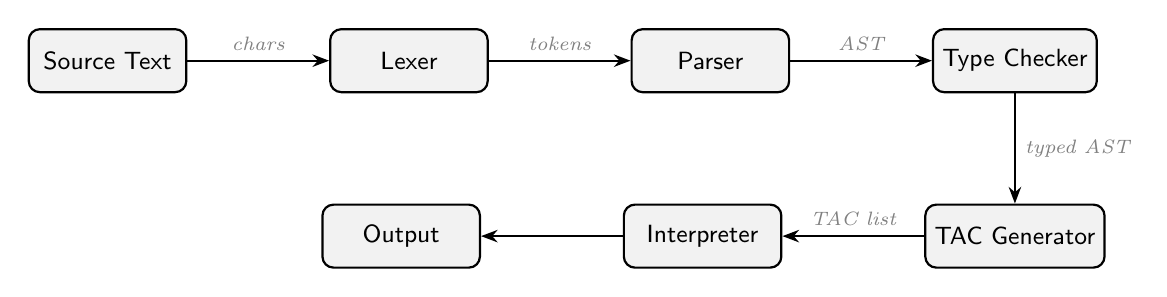
\begin{tikzpicture}[node distance=0.8cm and 1.8cm]

  % Row 1: Source -> Lexer -> Parser -> Type Checker
  \node[pipenode] (src) {Source Text};
  \node[pipenode, right=of src] (lex) {Lexer};
  \node[pipenode, right=of lex] (par) {Parser};
  \node[pipenode, right=of par] (tc)  {Type Checker};

  % Row 2: TAC Generator -> Interpreter -> Output
  \node[pipenode, below=1.4cm of tc]  (tac) {TAC Generator};
  \node[pipenode, left=of tac]        (int) {Interpreter};
  \node[pipenode, left=of int]        (out) {Output};

  % Row 1 arrows
  \draw[arrow] (src.east) -- node[annot, above] {chars}   (lex.west);
  \draw[arrow] (lex.east) -- node[annot, above] {tokens}  (par.west);
  \draw[arrow] (par.east) -- node[annot, above] {AST}     (tc.west);

  % Turn arrow
  \draw[arrow] (tc.south) -- node[annot, right] {typed AST} (tac.north);

  % Row 2 arrows
  \draw[arrow] (tac.west) -- node[annot, above] {TAC list} (int.east);
  \draw[arrow] (int.west) -- (out.east);

\end{tikzpicture}
\caption{The compilation pipeline}
\label{fig:pipeline}
\end{figure}

\section{Design Goals}

The language was designed with three explicit goals derived from the course
specification:

\begin{enumerate}
  \item \textbf{Static, inferred typing.} Every variable has a fixed type
        that is determined at compile time from its first assignment; no type
        annotations are written by the programmer.
  \item \textbf{No overloading.} Separate operator symbols for integer, float,
        and string operations eliminate ambiguity and make type inference
        purely syntax-directed.
  \item \textbf{Clarity of the intermediate representation.} Three-address code
        is generated as an explicit, human-readable intermediate form before
        execution, thereby separating code generation from interpretation.
\end{enumerate}

% =============================================================================
\chapter{Language Overview}
% =============================================================================

\section{Types}

The language provides four primitive types. There are no compound or
user-defined types.

\begin{table}[H]
\centering
\caption{Primitive types supported by the language.}
\label{tab:types}
\begin{tabular}{llp{5cm}}
\toprule
\textbf{Keyword} & \textbf{Type} & \textbf{Example Literals} \\
\midrule
\texttt{int}    & Integer          & \texttt{0}, \texttt{42}, \texttt{-7} \\
\texttt{float}  & Floating-point   & \texttt{3.14}, \texttt{0.5}, \texttt{100.0} \\
\texttt{bool}   & Boolean          & \texttt{true}, \texttt{false} \\
\texttt{string} & Character string & \texttt{"hello"}, \texttt{"world"} \\
\bottomrule
\end{tabular}
\end{table}

Variables are not declared explicitly. A variable's type is inferred from its
first assignment and remains fixed for the rest of its scope (see
Section~\ref{sec:typesystem}).

\section{Operators and Precedence}

The absence of overloading is the defining syntactic property of the language.
Each domain has its own operator symbols, and the grammar enforces the correct
domain at parse time.

\begin{table}[H]
\centering
\caption{Operator families grouped by domain and precedence.}
\label{tab:operators}
\begin{tabular}{@{} l l l c @{}}
\toprule
\textbf{Operators} & \textbf{Domain} & \textbf{Result} & \textbf{Prec.} \\
\midrule
\texttt{*}~\texttt{/}     & \tint{} $\times$ \tint{}       & \tint    & high \\
\texttt{+}~\texttt{-}     & \tint{} $\times$ \tint{}       & \tint    & low \\
\texttt{*.}~\texttt{/.}   & \tfloat{} $\times$ \tfloat{}   & \tfloat  & high \\
\texttt{+.}~\texttt{-.}   & \tfloat{} $\times$ \tfloat{}   & \tfloat  & low \\
\texttt{\^{}}              & \tstring{} $\times$ \tstring{} & \tstring & low \\
\texttt{=}~\texttt{<>}    & $\tau \times \tau$              & \tbool   & n/a \\
\bottomrule
\end{tabular}
\end{table}

Multiplication and division bind more tightly than addition and subtraction,
following standard mathematical convention. Comparison operators are
non-associative: writing \texttt{a = b = c} is a syntax error, which enforces
the specification requirement that boolean expressions compare exactly two
arithmetic expressions.

\section{Statements}

\begin{description}[style=nextline, leftmargin=2.5cm, labelwidth=2.3cm]
  \item[Assignment] \texttt{x = expr;}
        \hfill The first occurrence infers the variable's type.
  \item[If-then-else] \texttt{if bexpr then \{ \ldots \} else \{ \ldots \};}
  \item[While] \texttt{while bexpr do \{ \ldots \};}
  \item[Print] \texttt{print(expr);}
        \hfill Accepts any type.
  \item[Return] \texttt{return expr;}
        \hfill Valid only inside a function body.
\end{description}

\section{Functions}

Functions are declared before top-level statements using the \texttt{def}
keyword. Parameters are passed \emph{by value}: the callee receives a copy of
each argument, so assignments to parameters inside the function body have no
effect on the caller. Recursion is fully supported.

\begin{lstlisting}[caption={Function declaration syntax.}]
def int factorial(int n) {
    if n = 0 then { return 1; } else {
        return n * factorial(n - 1);
    };
}
\end{lstlisting}

% =============================================================================
\chapter{Grammar}
% =============================================================================

\section{Design Principles}

The grammar was designed so that:
\begin{itemize}
  \item Operator precedence is encoded structurally through grammar layering
        (\texttt{expr} $\to$ \texttt{term} $\to$ \texttt{atom}), with no
        need for external precedence declarations in the parser.
  \item Boolean expressions (\texttt{bexpr}) form a distinct nonterminal from
        arithmetic expressions (\texttt{expr}), making it syntactically
        impossible to use a comparison result as an arithmetic operand.
  \item The grammar is LALR(1): it can be parsed by a one-token-lookahead
        shift--reduce parser with no ambiguity.
\end{itemize}

\section{Complete Context-Free Grammar}

\begin{lstlisting}[style=tacstyle, numbers=none,
  caption={Complete grammar of PL (BNF notation).}]
program    -> def_list stmt_list

def_list   -> def def_list  |  (empty)

def        -> DEF type ID ( param_list ) { stmt_list }
            | DEF type ID (            ) { stmt_list }

param_list -> type ID , param_list  |  type ID

type       -> INT | FLOAT | BOOL | STRING

stmt_list  -> stmt ; stmt_list  |  (empty)

stmt       -> ID = bexpr
            | IF bexpr THEN { stmt_list } ELSE { stmt_list }
            | WHILE bexpr DO { stmt_list }
            | PRINT ( bexpr )
            | RETURN bexpr

bexpr      -> expr = expr
            | expr <> expr
            | expr

expr       -> expr +  term        (* integer addition       *)
            | expr -  term        (* integer subtraction    *)
            | expr +. term        (* float addition         *)
            | expr -. term        (* float subtraction      *)
            | expr ^  term        (* string concatenation   *)
            | term

term       -> term *  atom        (* integer multiplication *)
            | term /  atom        (* integer division       *)
            | term *. atom        (* float multiplication   *)
            | term /. atom        (* float division         *)
            | atom

atom       -> INT_LIT | FLOAT_LIT | STRING_LIT
            | TRUE | FALSE
            | ID
            | ID ( arg_list )  |  ID ( )
            | ( bexpr )

arg_list   -> bexpr , arg_list  |  bexpr
\end{lstlisting}

\section{Lexical Specification}

The lexer is built with \textbf{sly} using regular expressions. Token rules
are declared in priority order because \textit{sly} applies longest-match and
declaration-order disambiguation.

\begin{table}[H]
\centering
\caption{Token definitions and their regular expressions.}
\label{tab:tokens}
\begin{tabular}{@{} l l @{}}
\toprule
\textbf{Token} & \textbf{Regular Expression} \\
\midrule
\texttt{FLOAT\_LIT}  & \verb|[0-9]+\.[0-9]+| \\
\texttt{INT\_LIT}    & \verb|[0-9]+| \\
\texttt{STRING\_LIT} & \verb|"([^"\\]|\\.)*"| \\
\texttt{ID}          & \verb|[A-Za-z][A-Za-z0-9_]*| \\
\texttt{FPLUS}, \texttt{FMINUS}, etc. & \verb|\+\.| , \verb|-\.| , \verb|\*\.| , \verb|/\.| \\
\texttt{NE}          & \verb|<>| \\
Comments             & \verb|#.*| (discarded) \\
\bottomrule
\end{tabular}
\end{table}

\textbf{Priority notes.}
\texttt{FLOAT\_LIT} is declared before \texttt{INT\_LIT} so that
\texttt{3.14} is tokenised as a single float token rather than
\texttt{INT(3)}, \texttt{DOT}, \texttt{INT(14)}. Similarly, dotted operators
(\texttt{+.}) are declared before their plain counterparts (\texttt{+}) so
that the longer match wins. Keywords (\texttt{if}, \texttt{while},
\texttt{def}, etc.) are recognised by matching \texttt{ID} first and then
reclassifying the token if it appears in the keyword table---the standard
\textit{lex} idiom.

% =============================================================================
\chapter{Type System and Type Inference}
\label{sec:typesystem}
% =============================================================================
 
\section{Motivation}
 
The specification imposes two requirements that are in tension:
\emph{static} typing (all types must be known before execution) and \emph{no
explicit declarations} (the programmer never writes a type annotation for a
variable). The solution is \textbf{type inference}: the compiler figures out
each variable's type automatically by looking at how the variable is used.
 
Because every operator in PL has exactly one fixed signature (no overloading),
the type checker can determine all types in a single pass over the AST.
There is no need for complex algorithms like unification or constraint solving.
 
\section{Type Environments}
 
The type checker keeps track of types using two data structures:
 
\begin{itemize}
  \item \textbf{Variable environment} (a scoped stack of dictionaries):
        each dictionary maps variable names to their types. The global scope
        sits at the bottom of the stack. When the checker enters a function
        body, it pushes a new (empty) scope; when it leaves, it pops that
        scope. This gives correct scoping: variables inside a function cannot
        affect the caller's variables.
  \item \textbf{Function environment} (a single dictionary): maps each
        function name to its return type and the list of parameter types.
        For example, after seeing
        \texttt{def int factorial(int n)}, the entry would store
        return type = \tint{} and parameters = [\tint].
\end{itemize}
 
\section{Algorithm}
 
The algorithm works in two passes over the program AST.
 
\paragraph{Pass~1: Collect function signatures}
Before checking any function body, the type checker scans every \texttt{def}
node and records the function's return type and parameter types in the
function environment. This step is done first so that mutually recursive
functions work: the body of \texttt{f} can call \texttt{g} and vice versa,
because both signatures are already known.
 
\paragraph{Pass~2: Check bodies and annotate types}
Each function body is checked with a fresh variable scope that already
contains the function's parameters. The top-level statements are checked in
the global scope. During this pass, every expression node in the AST gets
a \texttt{.type} attribute attached to it, so the TAC generator can later
read the types directly without recalculating them.
 
\section{Type Checking Rules}
 
This section describes how the type checker determines the type of each
kind of expression and validates each kind of statement.
 
\subsection{Literals}
 
The type of a literal is determined directly from its syntax.
Table~\ref{tab:literal-types} summarises the mapping.
 
\begin{table}[H]
\centering
\caption{Type assigned to each literal form.}
\label{tab:literal-types}
\begin{tabular}{@{} l l l @{}}
\toprule
\textbf{Literal form} & \textbf{Example} & \textbf{Assigned type} \\
\midrule
Integer number   & \texttt{42}      & \tint    \\
Decimal number   & \texttt{3.14}    & \tfloat  \\
Quoted text      & \texttt{"hello"} & \tstring \\
\texttt{true} / \texttt{false} & \texttt{true} & \tbool \\
\bottomrule
\end{tabular}
\end{table}
 
\subsection{Variables}
 
When a variable name appears in an expression, the type checker looks it up
in the variable environment. If the variable has been assigned before, its
stored type is used. If the variable has never been assigned, the type
checker reports an error (``use before assignment'').
 
\subsection{Assignment and Type Inference}
 
Assignment is where type inference happens. There are two cases:
 
\begin{enumerate}
  \item \textbf{First assignment} (variable is new): the type checker
        evaluates the type of the right-hand side and records that type for
        the variable. For example, \texttt{x = 42;} causes \texttt{x} to be
        recorded as \tint.
  \item \textbf{Subsequent assignment} (variable already exists): the
        right-hand side must have the same type as the variable's recorded
        type. For example, after \texttt{x = 42;}, writing \texttt{x = "hi";}
        is a type error because \tstring{} does not match \tint.
\end{enumerate}
 
\subsection{Arithmetic Operators}
 
Each operator family requires specific operand types and produces a specific
result type. Table~\ref{tab:op-types} lists all operator families.
 
\begin{table}[H]
\centering
\caption{Type requirements for each operator family.}
\label{tab:op-types}
\begin{tabular}{@{} l l l @{}}
\toprule
\textbf{Operators} & \textbf{Required operand types} & \textbf{Result type} \\
\midrule
\texttt{+}~\texttt{-}~\texttt{*}~\texttt{/}       & both \tint   & \tint    \\
\texttt{+.}~\texttt{-.}~\texttt{*.}~\texttt{/.}    & both \tfloat & \tfloat  \\
\texttt{\^{}}                                       & both \tstring & \tstring \\
\bottomrule
\end{tabular}
\end{table}
 
Because there is no overloading, the operator itself tells the type checker
exactly what types to expect. For example, seeing \texttt{+} means both
operands must be \tint; seeing \texttt{+.} means both must be \tfloat.
If the operands do not match, a type error is raised.
 
\subsection{Comparison Expressions}
 
The comparison operators \texttt{=} (equality) and \texttt{<>} (inequality)
take two operands of the same arithmetic type (both \tint{} or both \tfloat)
and always produce a \tbool{} result. Comparing values of different types,
or comparing \tstring{} or \tbool{} values, is a type error.
 
\subsection{Control-Flow Statements}
 
For both \texttt{if-then-else} and \texttt{while-do}, the condition expression
must have type \tbool. If a non-boolean expression is used as the condition
(for example, \texttt{if 42 then \{...\}}), the type checker reports an
error. The statements inside the branches or loop body are checked recursively
using the same rules.
 
\subsection{Function Calls and Return}
 
When the type checker encounters a function call like \texttt{f(a, b)}, it:
\begin{enumerate}
  \item Looks up \texttt{f} in the function environment to find its expected
        parameter types and return type.
  \item Checks that the number of arguments matches the number of parameters.
  \item Checks that each argument's type matches the corresponding
        parameter's type.
  \item Assigns the function's declared return type as the type of the
        call expression.
\end{enumerate}
 
For \texttt{return} statements inside a function body, the type checker
verifies that the returned expression's type matches the function's declared
return type.
 
\section{Static Errors Detected}
 
The type checker raises a \texttt{TypeErrorException} for each of the
following violations, halting compilation before any code is generated:
 
\begin{itemize}
  \item Use of a variable before its first assignment.
  \item Reassignment of a variable with a value of a different type.
  \item Application of an operator to operands of the wrong type
        (e.g.,\ \texttt{1 +. 2} applies a float operator to integer literals).
  \item Comparison of values of different types, or comparison of
        non-arithmetic values (\tstring{} or \tbool).
  \item Calling a function with the wrong number of arguments or with
        arguments of incorrect types.
  \item A \texttt{return} expression whose type differs from the function's
        declared return type.
  \item A non-\tbool{} expression used as an \texttt{if} or \texttt{while}
        condition.
\end{itemize}
% =============================================================================
\chapter{Implementation}
% =============================================================================

\section{Module Structure}

Figure~\ref{fig:modules} shows the dependency graph among the six source
modules in the \texttt{src/} directory.

\begin{figure}[H]
\centering
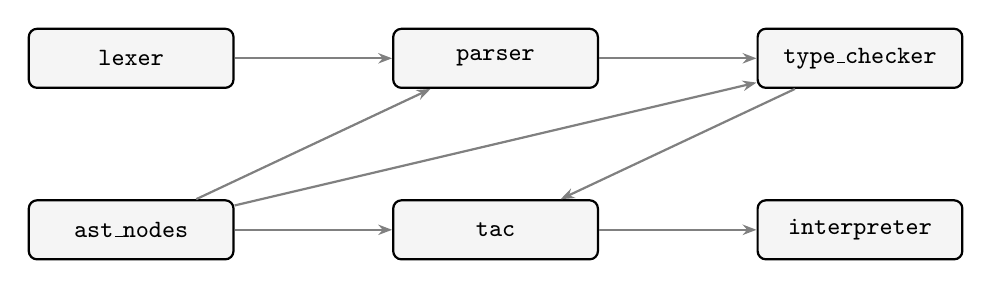
\begin{tikzpicture}[
  mod/.style={rectangle, draw=black, thick, rounded corners=3pt,
              minimum width=2.6cm, minimum height=0.75cm,
              font=\small\ttfamily, fill=gray!8},
  dep/.style={-{Stealth[length=5pt]}, thick, gray},
  node distance=1.4cm and 2.0cm,
]
  % Row 1
  \node[mod] (lex)  {lexer};
  \node[mod, right=of lex]  (par)  {parser};
  \node[mod, right=of par]  (tc)   {type\_checker};

  % Row 2
  \node[mod, below=of lex]   (ast)   {ast\_nodes};
  \node[mod, below=of par]   (tac)   {tac};
  \node[mod, below=of tc]    (interp){interpreter};

  % Arrows (dependency -> dependent)
  \draw[dep] (lex)   -- (par);
  \draw[dep] (par)   -- (tc);
  \draw[dep] (ast)   -- (par);
  \draw[dep] (ast)   -- (tc);
  \draw[dep] (ast)   -- (tac);
  \draw[dep] (tc)    -- (tac);
  \draw[dep] (tac)   -- (interp);

\end{tikzpicture}
\caption{Module dependency graph}
\label{fig:modules}
\end{figure}

\section{Lexer}

The lexer (\texttt{src/lexer.py}) is implemented using \textbf{sly}. Each
token type is declared as a class attribute holding either a string (for a
regular expression) or a dictionary (for the keyword remap table). The
\texttt{ignore} and \texttt{ignore\_comment} attributes silently discard
whitespace and \texttt{\#}-comments.

\section{Parser}

The parser (\texttt{src/parser.py}) is a \textit{sly} LALR(1) parser. Grammar
productions are written as Python methods decorated with \texttt{@\_(...)}
where the argument is the production rule as a string.
Left-recursive rules for \texttt{expr} and \texttt{term} yield left-to-right
associativity for arithmetic operators.
Each action builds and returns an AST node; the root action returns a
\texttt{Program} node containing all function definitions and the
top-level statement list.

\section{Abstract Syntax Tree}

All AST nodes are Python \texttt{dataclass} instances defined in
\texttt{src/ast\_nodes.py}. Table~\ref{tab:ast} lists every node type.

\begin{table}[H]
\centering
\caption{AST node types and their fields.}
\label{tab:ast}
\begin{tabular}{@{} l l l @{}}
\toprule
\textbf{Category} & \textbf{Node} & \textbf{Fields} \\
\midrule
Literals    & \texttt{IntLit}, \texttt{FloatLit},
            & \texttt{value} \\
            & \texttt{StringLit}, \texttt{BoolLit} & \\
\addlinespace
Expressions & \texttt{Var}    & \texttt{name} \\
            & \texttt{BinOp}  & \texttt{op, left, right} \\
            & \texttt{Compare}& \texttt{op, left, right} \\
            & \texttt{Call}   & \texttt{name, args} \\
\addlinespace
Statements  & \texttt{Assign} & \texttt{name, expr} \\
            & \texttt{If}     & \texttt{cond, then\_block, else\_block} \\
            & \texttt{While}  & \texttt{cond, body} \\
            & \texttt{Print}  & \texttt{expr} \\
            & \texttt{Return} & \texttt{expr} \\
\addlinespace
Top-level   & \texttt{FuncDef}& \texttt{return\_type, name, params, body} \\
            & \texttt{Program}& \texttt{funcs, main} \\
\bottomrule
\end{tabular}
\end{table}

\section{Three-Address Code Generator}

\subsection{Instruction Set}

The TAC generator (\texttt{src/tac.py}) traverses the annotated AST and emits
a flat list of instructions. Each instruction is a Python \texttt{dataclass}.
Table~\ref{tab:tac} lists the complete instruction set.

\begin{table}[H]
\centering
\caption{Three-address code instruction set.}
\label{tab:tac}
\small
\begin{tabular}{@{} l l p{4.2cm} @{}}
\toprule
\textbf{Instruction} & \textbf{Fields} & \textbf{Semantics} \\
\midrule
\texttt{Assign}    & \texttt{dest, src}         & $\mathit{dest} \leftarrow \mathit{src}$ \\
\texttt{BinOp}     & \texttt{dest, op, l, r}    & $\mathit{dest} \leftarrow l\ \mathit{op}\ r$ \\
\texttt{Label}     & \texttt{name}              & Jump target. \\
\texttt{Jump}      & \texttt{label}             & Unconditional jump. \\
\texttt{JumpIf}    & \texttt{cond, label}       & Jump if true. \\
\texttt{JumpIfNot} & \texttt{cond, label}       & Jump if false. \\
\texttt{Param}     & \texttt{arg}               & Push call argument. \\
\texttt{Call}      & \texttt{dest, func, n}     & $\mathit{dest} \leftarrow \mathit{func}(\ldots)$ \\
\texttt{Return}    & \texttt{val}               & Return to caller. \\
\texttt{Print}     & \texttt{val}               & Emit to output. \\
\texttt{FuncBegin} & \texttt{name}              & Prologue marker. \\
\texttt{FuncEnd}   & \texttt{name}              & Epilogue marker. \\
\bottomrule
\end{tabular}
\end{table}

Temporaries are named \texttt{t0}, \texttt{t1}, \ldots{} using a global
counter, which guarantees uniqueness across the whole program. Labels use the
same scheme: \texttt{L0}, \texttt{L1}, \ldots{}

Each literal value is wrapped in a \texttt{Lit(value)} container before
it is stored in an \texttt{Assign.src} field, distinguishing it from
variable or temporary names (which are plain strings).
Without this wrapper, the string literal \texttt{"world"} would be
indistinguishable from a variable named~\texttt{world}.

\subsection{Control-Flow Translation Schemes}

\textbf{If-then-else} is translated to a conditional branch around the
then-block and an unconditional jump over the else-block:

\begin{lstlisting}[style=tacstyle, numbers=none]
    <evaluate condition into t_c>
    ifnot t_c goto L_else
    <then-block instructions>
    goto L_end
L_else:
    <else-block instructions>
L_end:
\end{lstlisting}

\textbf{While} is translated with the condition check at the top of the loop:

\begin{lstlisting}[style=tacstyle, numbers=none]
L_test:
    <evaluate condition into t_c>
    ifnot t_c goto L_end
    <body instructions>
    goto L_test
L_end:
\end{lstlisting}

\textbf{Function calls} use the \texttt{param}/\texttt{call} protocol:

\begin{lstlisting}[style=tacstyle, numbers=none]
    param a_1
    param a_2
    ...
    t_r = call f [n]     (* n = number of arguments *)
\end{lstlisting}

\section{Interpreter}

The interpreter (\texttt{src/interpreter.py}) executes the flat TAC list
using a \textbf{program counter} (PC) that indexes into the instruction array.

\paragraph{Startup scan}
Before execution begins, the interpreter makes a single pass over all
instructions to build two lookup tables:
\begin{itemize}
  \item \texttt{label\_map}: label name $\mapsto$ instruction index.
  \item \texttt{func\_map}: function name $\mapsto$ index of the first
        instruction following its \texttt{FuncBegin}.
\end{itemize}

\paragraph{Main-body execution}
The main body is located by finding the index immediately after the last
\texttt{FuncEnd} instruction. Execution then enters the dispatch loop.
If a \texttt{FuncBegin} is encountered during main-body execution
(which would happen in the pathological case of an empty function list or
a mid-stream jump error), the interpreter fast-forwards past the matching
\texttt{FuncEnd}.

\paragraph{Function-call dispatch}
When a \texttt{Call} instruction is executed:
\begin{enumerate}
  \item The required number of values is popped from the \texttt{pending\_params}
        list that was accumulated by preceding \texttt{Param} instructions.
  \item A fresh environment \emph{frame} (a Python dictionary) is created and
        populated with the mapping from parameter names to argument values.
        Parameter names are recovered from the original AST via a
        side-table built at startup.
  \item The interpreter recursively calls \texttt{\_exec} starting at
        \texttt{func\_map[f]}. Because the frame is entirely separate from
        the caller's environment, this constitutes pure value-parameter passing.
\end{enumerate}

\paragraph{Operator evaluation}
Table~\ref{tab:opsem} lists the Python semantics used for each operator
in the interpreter.

\begin{table}[H]
\centering
\caption{Operator semantics in the interpreter.}
\label{tab:opsem}
\begin{tabular}{@{} l l @{}}
\toprule
\textbf{Operator} & \textbf{Python Semantics} \\
\midrule
\texttt{+}~\texttt{-}~\texttt{*} & \texttt{int} arithmetic \\
\texttt{/}           & \texttt{l // r} (floor div.; error on zero) \\
\texttt{+.}~\texttt{-.}~\texttt{*.}~\texttt{/.} & \texttt{float} arithmetic \\
\texttt{\^{}}        & \texttt{str(l) + str(r)} \\
\texttt{=}           & \texttt{l == r} $\to$ \texttt{bool} \\
\texttt{<>}          & \texttt{l != r} $\to$ \texttt{bool} \\
\bottomrule
\end{tabular}
\end{table}

% =============================================================================
\chapter{Example Programs and Traces}
% =============================================================================

This chapter presents five programs that exercise every language feature.
Each example is followed by a type-checking analysis and, where appropriate,
the generated three-address code.

\section{Recursive Factorial}

\begin{lstlisting}[caption={Recursive factorial function.}]
def int factorial(int n) {
    if n = 0 then { return 1; } else {
        return n * factorial(n - 1);
    };
}

n      = 6;
result = factorial(n);
print(result);
\end{lstlisting}

The type checker verifies the following:
\begin{itemize}
  \item Parameter \texttt{n} has type \tint{} (declared).
  \item \texttt{n = 0}: comparison of two \tint{} expressions; the result is
        \tbool{}---a valid condition.
  \item \texttt{n * factorial(n - 1)}: both operands are \tint{}, and operator
        \texttt{*} produces \tint{}, which matches the declared return type.
\end{itemize}

Generated TAC for the function body:

\begin{lstlisting}[style=tacstyle, caption={TAC for \texttt{factorial}.}]
--- function factorial ---
    t0 = 0
    t1 = n = t0
    ifnot t1 goto L0
    t2 = 1
    return t2
    goto L1
L0:
    t3 = 1
    t4 = n - t3
    param t4
    t5 = call factorial [1]
    t6 = n * t5
    return t6
L1:
--- end factorial ---
\end{lstlisting}

\section{Iterative While Loop}

\begin{lstlisting}[caption={Computing the sum $1 + 2 + \cdots + 5$ iteratively.}]
i   = 1;
sum = 0;
while i <> 6 do {
    sum = sum + i;
    i   = i + 1;
};
print(sum);   # prints 15
\end{lstlisting}

Both \texttt{i} and \texttt{sum} are inferred as \tint{} from their first
assignments. The condition \texttt{i <> 6} compares two \tint{} values,
yielding \tbool{}---a valid \texttt{while} condition.

\section{Float Arithmetic}

\begin{lstlisting}[caption={Celsius-to-Fahrenheit conversion.}]
def float to_fahrenheit(float c) {
    return c *. 1.8 +. 32.0;
}

temp = to_fahrenheit(100.0);
print(temp);   # prints 212.0
\end{lstlisting}

The expression \texttt{c *. 1.8 +. 32.0} is evaluated left to right:
\texttt{c *. 1.8} has type \tfloat{} (multiplication takes precedence),
and then \texttt{+. 32.0} adds a \tfloat{} literal---the expression is
type-correct throughout.

\section{String Concatenation}

\begin{lstlisting}[caption={String concatenation with the \texttt{\^{}} operator.}]
first = "hello";
last  = "world";
msg   = first ^ ", " ^ last ^ "!";
print(msg);   # prints hello, world!
\end{lstlisting}

\section{Type Error Detection}

The following program is rejected at the type-checking phase before any code
is generated:

\begin{lstlisting}[caption={Program rejected by the type checker.}]
x = 1 +. 2;
\end{lstlisting}

The compiler produces the following error message:

\begin{lstlisting}[style=errorstyle]
Type error: operator '+.' requires float operands,
            got 'int' and 'int'.
\end{lstlisting}

% =============================================================================
\chapter{Online Compiler}
% =============================================================================

A browser-based compiler interface is included in the \texttt{web/} directory,
providing access to the full pipeline without any local installation.\footnote{Live demo: \url{https://pl-compiler.ambitiousisland-1be3b1ed.southeastasia.azurecontainerapps.io/}} The
architecture is described below.

\paragraph{Backend}
A \textbf{Flask} application (\texttt{web/app.py}) exposes two HTTP
endpoints. \texttt{GET /} serves the single-page UI.
\texttt{POST /run} accepts a JSON body containing the source text and a
boolean \texttt{show\_tac} flag, runs the full pipeline with standard output
redirected to a string buffer, and returns the captured output (or an error
message) as JSON.

\paragraph{Frontend}
The single-page interface (\texttt{web/templates/index.html}) is built with
plain HTML, CSS, and JavaScript. It embeds \textbf{CodeMirror~5} (loaded from
a CDN) as the code editor, providing syntax highlighting, line numbers, and
bracket matching. A \emph{Load Example} dropdown populates the editor with any
program from the \texttt{examples/} directory. Pressing \textbf{Run} (or
\texttt{Ctrl+Enter}) sends the editor contents to \texttt{/run} via the
Fetch~API and displays the result in the output pane. The \emph{Show TAC}
checkbox switches the output pane to display the generated three-address code
instead of the program's runtime output.

% =============================================================================
\chapter{Conclusion}
% =============================================================================

This report has presented the design and implementation of a complete,
statically typed programming language built in approximately 600~lines of
Python across six modules. The language supports four primitive types
(\tint, \tfloat, \tbool, and~\tstring), first-assignment type inference,
arithmetic and boolean expressions without operator overloading, the standard
imperative control structures (assignment, if-then-else, and while-do), and
user-defined functions with value-parameter passing.

The implementation follows a classical compilation pipeline: lexical analysis
tokenises the source text, an LALR(1) parser builds an abstract syntax tree,
a two-pass type checker infers and validates all types, a code generator
emits three-address code as an explicit intermediate representation, and an
interpreter executes the resulting instruction sequence. Each stage is
encapsulated in its own module, keeping the architecture clear and
maintainable.

Beyond the core pipeline, the project includes a browser-based online
compiler that allows users to write, compile, and run programs without any
local installation, as well as a structured set of example programs that
exercise every language feature independently.

\end{document}